\documentclass[10pt,a4paper]{article}
\usepackage[latin1]{inputenc}
\usepackage{amsmath}
\usepackage{amsfonts}
\usepackage{amssymb}
\usepackage{graphicx}
\usepackage{amsthm}
\graphicspath{{images/}}

\newcommand{\R}{\mathbb{R}}

\begin{document}

\theoremstyle{definition}
\newtheorem{defn}{Definition}[section]


	\section{Basic definitions}

	\begin{defn}{Support}
		The set of values a random variable can take (set of all the numerical realizations of outcomes) e.g. for a binary random variable X, it's support is $R_X = \{ 0, 1 \}$
	\end{defn}


	\begin{defn}{Sample Point}
		In an experiment, a sample point is one of the possible outcomes of experiment denoted by $\omega$
	\end{defn}

	\begin{defn}{Independent Events}
	Two events A and B are independent if and only if \\
	\begin{align}
		P(A \cap B) = P(A) * P(B)
	\end{align}
	\end{defn}

	\begin{defn}{Jointly/Mutually Independent Events}
	Let $E_1, ... , E_n$ be n events. \\
	$E_1, ... , E_n$ are jointly independent(or mutually independent)
	if and only if for any sub-collection of k events $(k \leq n) E_{i1}, ... , E_{ik}$:
	\begin{align}
	P(\bigcap \limits_{j=1}^kE_{ij}) = \prod_{j=1}^{k}P(E_{ij})
	\end{align}
	\end{defn}

	\begin{defn}{Random Variable}
		A random Variable $X$ is a function from sample space $\Omega$ to set of real numbers $\R$, i.e $ X: \Omega -> \R $.\\
		
		The real number $X(\omega)$ associated with sample point $\omega \in \Omega$ is called a realization of the random variable. The set of all possible realizations is called the support and denoted by $R_X$
	\end{defn}

	\begin{defn}{Probability Mass Function}
		The PMF of a discrete random variable $X$ is a function $p_X : \R -> [0,1]$ such that\\
		$p_X = P(X = x)\quad \forall x \in \R$\\
		where $P(X = x)$ is the probability of realization of random variable X will be equal to x. Basically PMF is numerical realizations $->$ respective Probabilities.
	\end{defn}

	\begin{defn}{Distribution Function/Cumulative Distribution Function}
		If $X$ is a random variable, its distribution/cdf is a function $F_X : \R -> [0,1]$ such that \\
		\begin{align}
			F_X(x) = P(X \le x) \quad \forall x \in \R
		\end{align}
	\end{defn}

	\begin{defn}{Expected Value of a Random Variable}
	The expected value of random variable $X$ is the weighted average of the values that X can take on where each possible value is weighted by its respective probabilit i.e. \\
	\begin{align}
		E[X] = \sum\limits_{x \in R_X}xp_X(x)
	\end{align}
	\end{defn}

	\begin{defn}{Deviation of a Random Variable}
	The expected value of random variable $X$ is the weighted average of the values that X can take on where each possible value is weighted by its respective probabilit i.e. \\
	$E[X] = \sum\limits_{x \in R_X}xp_X(x)$
	\end{defn}

	\begin{defn}{Variance}
		It is a measure of dispersion of a random variable.
	\end{defn}

	\begin{defn}{Covariance}
	It is a measure of association between two random variables.
	Covariance of two random variables X and Y is , provided Expected values are well defined,
	\begin{equation}
		Cov[X,Y] = E[ (X - E[X]) * (Y - E[Y]) ] = E[\overline{X} * \overline{Y}]
	\end{equation}
	where we say deviation of X is $\overline{X} = X - E[X]$ and \\
	deviation of Y is $\overline{Y} = Y - E[Y]$\\
	or in other words, covariance is expectation of product of deviations.
	\end{defn}

	\begin{defn}{Random Vector}
	It is a multidimensional generalisation of the concept of Random Variable. Associated probability functions have the word "joint" in front of them e.g. Joint PMF, Joint cdf etc correspond to a Random Vector.
	\end{defn}

	\section{Logistic}	
	A logistic function or logistic curve is a common 'S' shaped curve with equation:
	
	\begin{equation}
			f(x) = \frac{L}{1 + e^{-k(x-x_0)}}
	\end{equation}

	
	where
	\begin{itemize}
		\item e = natural log
		\item $x_0$ = x-value of sigmoid's midpoint
		\item L = the curve's maximum value
		\item k = the steepness of the curve
	\end{itemize}

	\subsection{Standard Logistic}
	
	The standard logistic function is the logistic function with parameters given $(k = 1, x_0 = 0, L = 1)$
	i.e.\\
	\begin{equation}
		\sigma(x) = \frac{1}{1 + e^{-x}}
	\end{equation}
	which when plotted looks like\\
	\begin{figure}[h]
		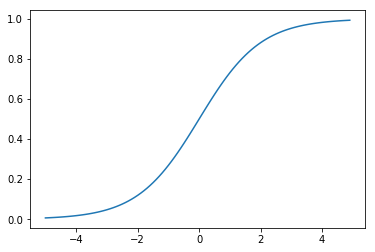
\includegraphics[scale=0.65]{sigmoidplot}
		\centering
	\end{figure}

	\textbf{Why is logistic function so important?}
	Because it can take any real input $x, (x \in R)$, whereas the output always takes values between 0 and 1, and hence is interpretable as probability.
	

	
\end{document}